\chapter{Related Work}
\label{ch:related_work}

The related literature can be split into two categories. Section~\ref{sec:classnews} is about the classification of news comments. While for some approaches consider the context, i.e., an article's title, it is only one feature among others. The comment is not considered embedded in a whole conversational context. This is different to approaches presented in Section~\ref{sec:contextawaretext}. There the exploitation of the sequential or tree-structures of online discussions is the principal motivation.

\section{Classification of News Comments}
\label{sec:classnews}

With the beginning of Web 2.0, there is an abundance of user-generated content freely accessible. Some influential earlier work analyzed comments on Digg\footnote{\url{https://digg.com}}~\cite{Gomez:2008:SAS:1367497.1367585, Lampe:2004:SBD:985692.985761}, or predicted the popularity of online content on YouTube\footnote{\url{https://youtube.com}} and Digg~\cite{Szabo:2010:PPO:1787234.1787254} or Reddit\footnote{\url{https://reddit.com}}~\cite{Rizos:2016:PNP:2872518.2890096}. The analysis of news comments is a subset of the research done on user-generated content so it falls in this line. But we focus on news comments so the remaining section is dedicated to them.

Coming from the area of Human-Computer Interaction (HCI), Park et al.~\cite{Park:2016:SCM:2858036.2858389} build an IT system to support moderators to identify high-quality comments. They incorporate traditional, feature-based machine learning. Besides other components, they automatically assign a quality score to each comment. They hand-crafted various features based on a comment's text as well as metadata. For instance, they consider a comment's text as well as the commentator's history. The authors tried to measure the distance of a comment's text to the article's text and other comments' text as \textit{relevance} of a comment. This relevance metric originates from work by Nicholas Diakopoulos~\cite{Diakopoulos:2015:EEC:2675133.2675160}. He uses a simple tf-idf~\cite{salton1986introduction} model to create vector representations of comments and articles to use, i.e., cosine distance to measure similarity amongst comments or between an article and a comment. This metric has serious short comings since it only considers identical words matches. So for instance, the heavy use of synonyms results in a comment to be marked as irrelevant to an article. However, for Park et al. the machine learning part is not the focus of their work. They simply demonstrate what can be built by applying NLP and machine learning to news comments. In this sense, well-functioning machine learning techniques, such as classification, are a necessity for those end-to-end systems. Park et al. conclude in their section that more research in the area is required.

A similar work by H\"aring et al.~\cite{haring2018addressed} focusses on the classification of German \textit{meta-comments}. Meta-comments are comments that, i.e., address an article's authors directly. So they are not about the topic of an article but \textit{meta}, so meta-comments. In cooperation with a large German newspaper, they highlight the need for journalists to identify those comments. Journalists only have a limited amount of time so they want to spend it wisely. For the classification, they experiment with various traditional manually engineered features. They also conduct qualitative research about identifying also characteristics of those meta-comments. The author's research is only touching machine learning with NLP since it is published at a HCI conference. They also tried to use neural models but traditional machine learning methods outperformed them. They conjecture that the number of annotated data with only a couple hundreds samples is too few. They do not use any conversation or context-aware methods. Only the news department of an articles is considered. Besides proprietary data, they use the research dataset \textit{One Million Posts} by Schabus et al.~\cite{Schabus:2017:OMP:3077136.3080711} consisting of Austrian comments. The authors constructed a dataset of one million unlabeled comments and annotated a view thousand of them. They present several approaches and experiment with feature-based machine learning as well as deep learning. On two out of eight categories a Long short-term memory network (LSTM)~\cite{Hochreiter:1997:LSM:1246443.1246450} achieved the best $\text{F}_{1}$ score. In their follow-up paper, Schabus and Skowron~\cite{schabus_academic-industrial_nodate} describe how they resort to a feature-based machine method for usage in a production system. They also experiment with including features related to the headline of category of the article but could not get good results. They focus on the implementation of a news comment classification system. While they report baselines, that point out that there are only baselines. Their $\text{F}_{1}$ scores range from about 0.15 (positive comments) to about 0.7 (personal stories) so there is still room for improvement. They also point out the difficulties of news comment classification since comments are much more ``diverse in terms of topic, style, length, author intention [..]'' than movie reviews. Detecting sentiment in movie reviews is a common problem setting for NLP research.

News organization realized that high-quality comments are easily overlooked in the vast amount of comments. Even though the community votes on comments, those comments with the most up-votes are not necessarily the ones with the highest quality. Thus, moderators pick comments themselves. On the New York Times\footnote{\url{https://www.nytimes.com}} (NYT) website,  those comments are called \textit{NYT Picks}. Since these comments went through a selection process, one can think about it as a binary classification problem. This caught the interest of research to investigate the characteristics of picked and non-picked comments. But in this kind of post-hoc analysis, it is hard to understand the reasoning process of the moderations and other external factors. It is also more than likely that different people picked and the selection process varied over the time. Altogether, this annotation process is very opaque. Nevertheless, research was working with it. Nicholas Diakopoulos~\cite{diakopoulos2015picking} presents nine criteria for comments that distinguish NYT Picks from non-NYT Picks and three of them can be computed: Brevity, Readability, and Personal Experience. For the other six, Diakopoulos paid crowd-annotators to classify them and found significant differences between picked and not picked ones. One finding is that comments are more likely to get picked shorty after the release of an article. However, this could also be explained with the selection process of moderators. Maybe they were following the debate in the comment section more closely in the beginning. The authors' work falls more into the area of communication but even there their finding are to question due to uncertainty around the selection process.

Kolhatkar and Taboada~\cite{kolhatkar_using_2017} try to automatically identify constructive comments. They define constructive as follow:
\begin{quote}
     ``Constructive comments intend to create a civil dialogue through remarks that are relevant to the article and not intended to merely provoke an emotional response. They are typically targeted to specific points and supported by appropriate evidence.''
\end{quote}
Since there is a scarcity of labeled annotated comments, they used the NYT picks in a creative way. They are aware of the fact that it is hard to draw conclusion from the non-picked comments. So they only consider the picked comments and define them as constructive. These are the positive samples. As negative, they resort to another dataset about news comments, the Yahoo News Annotated Comment Corpus (YNACC)~\cite{napoles2017finding}. The YNACC contains annotations on comment-level as well a thread-level. One category for the classification is constructiveness. So Kolhatkar and Taboada choose all comments from non-constructive threads as the negative samples.
They conduct experiments on several model variations. They report results on yet another set of annotated comments that they published as the SFU Opinion and Comments Corpus (SOCC)~\cite{kolhatkar2018sfu}.
However, they were mainly focusing on traditional feature-based machine learning. They were using some simple length features, e.g, comment length and average word length, and achieved an $\text{F}_{1}$ score of 0.79. They were unable to push the score further with more features. With other more complex features argumentation, text quality, and named entity features, they achieved an $\text{F}_{1}$ score of 0.84. They also investigated approaches based on deep learning, a bidirectional LSTM, and received a $\text{F}_{1}$ score of 0.81. The number of training samples with about 30k should be sufficient to outperform traditional machine learning. However, it did not beat the feature-based machine learning approaches on the test set. But their values are only on the SOCC dataset which is used as test set. And those comment stem from another newspaper than the comments the model was trained one. When looking at the validation set, the LSTM outperformances all other approaches with an $\text{F}_{1}$ score of 0.86 and 0.83 on the second place. The comments in the training and validation set are from the same newspaper.
So the results should be interpret carefully. In their follow-up work, Kolhatkar and Taboada~\cite{kolhatkar2017constructive} predicted the comments in the SOCC with an accuracy of $72.59\%$ by using an LSTM.
This must also be taken with caution since the number of samples is relatively low (1k).

The aforementioned YNACC dataset was in the focus of the work of Napoles et al.~\cite{napoles2017automatically}. They identified constructive threads among 2.4k annotated threads. The major focus of their work is traditional machine learning. They employ traditional feature engineering. Furthermore, they use features of the comment's text as well as features of the user such as commenting history and also user contributed up- and downvotes. They compare several results, also a neural model. The best performing model is a pipeline model that comprises several steps of features created from a comment's text as well as metadata. They achieve a $\text{F}_{1}$ score of 0.73 on the test set of the YNACC data and $\text{F}_{1}$ score of 0.91 on another external dataset of an online discussion forum. Even if the numbers on the external datasets sound impressing, no significance testing was applied. Since the datasets with about 1k samples is, once again, relatively low, the results may be created by chance. And it is not clear on how many different external datasets the model was tested. Maybe it was tested on 10 different datasets, and it performed well on only one datasets and so the results may be cherry-picked. Also it is not clear how difficult the classification of this external dataset it. Maybe a simple baseline could have achieved even better results. So while the paper shows the performance of certain features, the results have to be interpret carefully.

In this section, we briefly introduced research datasets of annotated news comments. A detailed comparison of all available datasets is presented in Section~\ref{sec:datasets_comments_table}.

\section{Conversation-aware Text Classification}
\label{sec:contextawaretext}

In this section, we present text classification approaches that exploit sequential or tree structures of text. This is often the case on social media platforms with their nested comment structures. The conversation is often started by a particle item, such as a news article or a social media post. This starts an online conversation where subsequent comments are part of this conversation.

Cheng et al.~\cite{2018arXiv180807191C}\footnote{This publication was not formally published and is only a pre-print. We still consider it relevant because it is recent and closely related to our (niche) topic.} consider the abstract of the news article as well as surrounding comments to classify comments. It adapts the text matching approach that uses an LSTM with attention mechanism. They describe text matching as a general problem to decide whether two text relate to each other in some way. In this sense, question answering or duplicate detection are a special case of a text matching. In this case, the text matching is done between a comment and surrounding comments as well as a comment and article's abstract and title. The text is represented by Word2vec embeddings~\cite{DBLP:journals/corr/abs-1301-3781}. The text matching computations are combined  in a final layer. Then then a comment gets classified. However, the paper has one weakness. They interpret all comments with over 10 up-votes as positive and the rest as negative samples in a binary classification problem. This is a gross simplification. For instance, earlier comments are more likely to get more up-votes. So they may only predict comments that appear earlier in the discussions than others. Furthermore, certain topics attract more people and thus receive more votes. So there is no justification for the number of 10 up-votes. In order to use the votes as labels, one has to normalize the up-votes and down-votes. The social media platform Reddit has implemented a system to normalize upvotes since time since posted. Even though the authors achieved an accuracy of $70.75\%$ and a $\text{F}_{1}$ score of $0.8073$, their true contribution is unclear.

\newpage

Covering the related work on hate speech detection is out of scope for this paper. But there is one particular paper by Gao and Huang~\cite{Gao_2017} that is closely related because they work on context-aware classification.
They as well point out that work on comments neglects its context. They developed an architecture of three parallel LSTMs, one for the text, one for the author, and one for the article. Those three LSTMs are combined into a final layer before classifying. They as well used pre-trained Word2vec embeddings for text representation. They constructed their own datasets of annotated tweets that relate to news articles. In their experiments, they claim that their context-aware model outperforms the one without context. Unfortunately, they did not apply their method to a commonly used dataset to put their contribution into perspective.
 \begin{figure}
  \begin{center}
    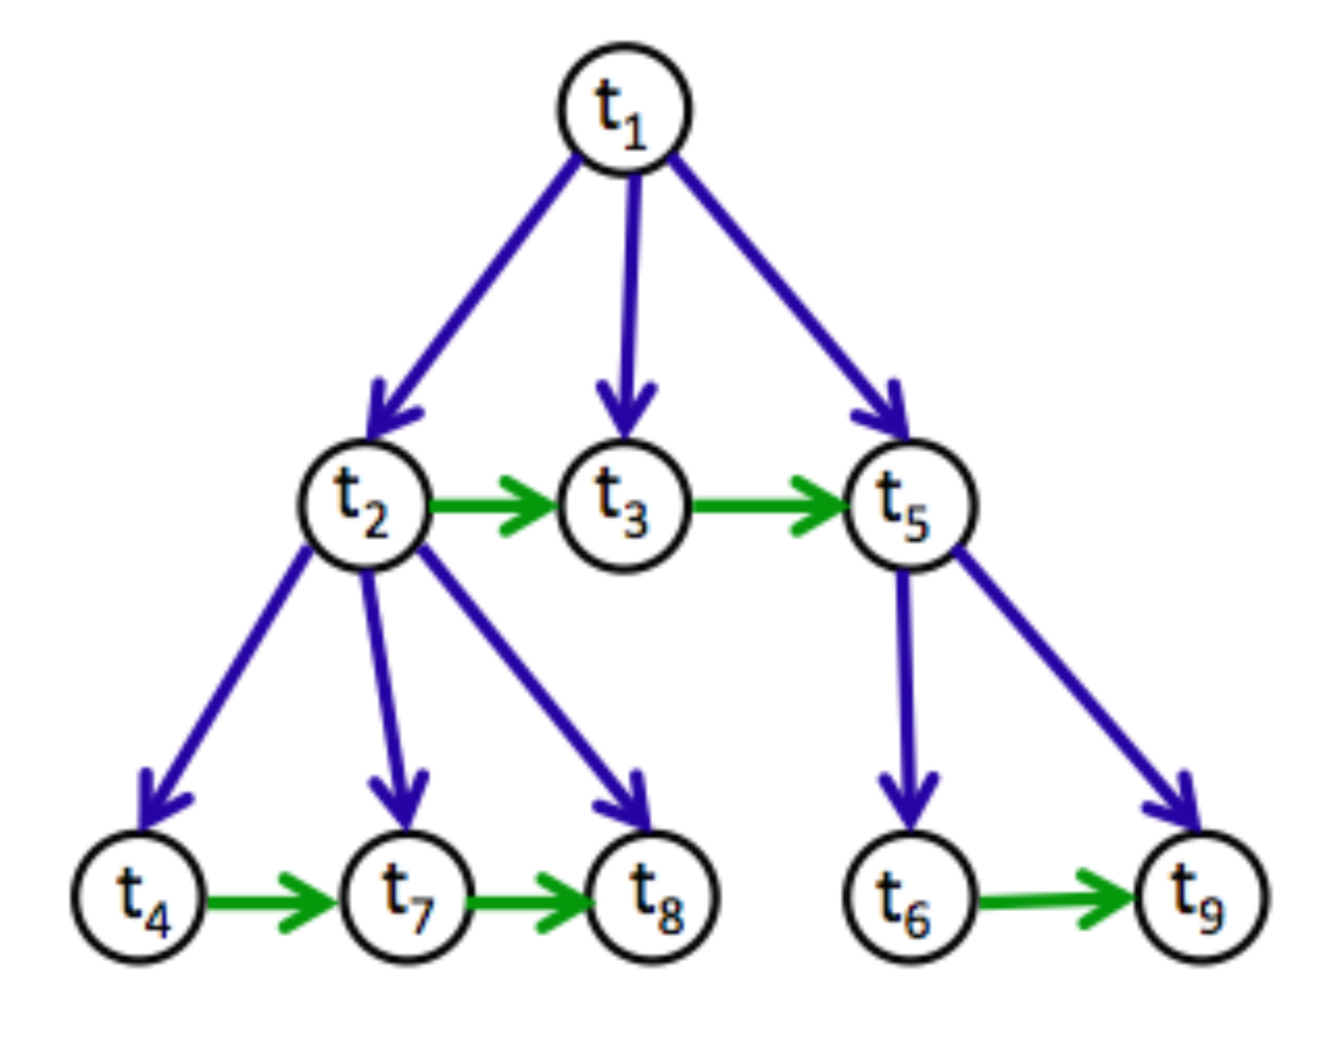
\includegraphics[width=0.4\textwidth]{images/related_work/conversial_modelling.png}
  \end{center}
  \caption{The Graph structure gets introduced to the LSTM with two different previous time steps. The figures is taken from the original paper by Zayats and Ostendorf~\cite{Q18-1009}.}
   \label{fig:zayats_tree} 
\end{figure}

A new LSTM cell by Zayats and Ostendorf~\cite{Q18-1009} intends to exploit the graph structure of the data. They add an additional previous time step. So there is one previous time step for the hierarchy and one for the time. The two different steps are illustrated in Figure~\ref{fig:zayats_tree}.
 To evaluate their contribution, they predict community votings on Reddit comments. With their approach, they outperformed context-agnostic approaches in their work. To represent their text, they used Word2vec embeddings. They did not evaluate their approach on other text classification tasks. Since the votings has some uncertainties as already mentioned earlier, the benefit of this LSTM modification is uncertain. Miura et al.~\cite{C18-1322} conducted additional experiments with this LSTM cell. But they used Reddits comments that were annotated for their role in the discourse.
 The dataset is named Coarse Discourse~\cite{coarsediscourse} and it will be described in the next paragraph.
So it was different setup and the results were below other more traditional machine learning approach of a conditional random field. They hypotheses that predicting user votes is a special kind of problem setting where the text is not a major factor. Other features such as the timing of a comment plays is more important. So this cell is not suited for text classification and thus not for news comments classification.
\begin{figure}
  \begin{center}
    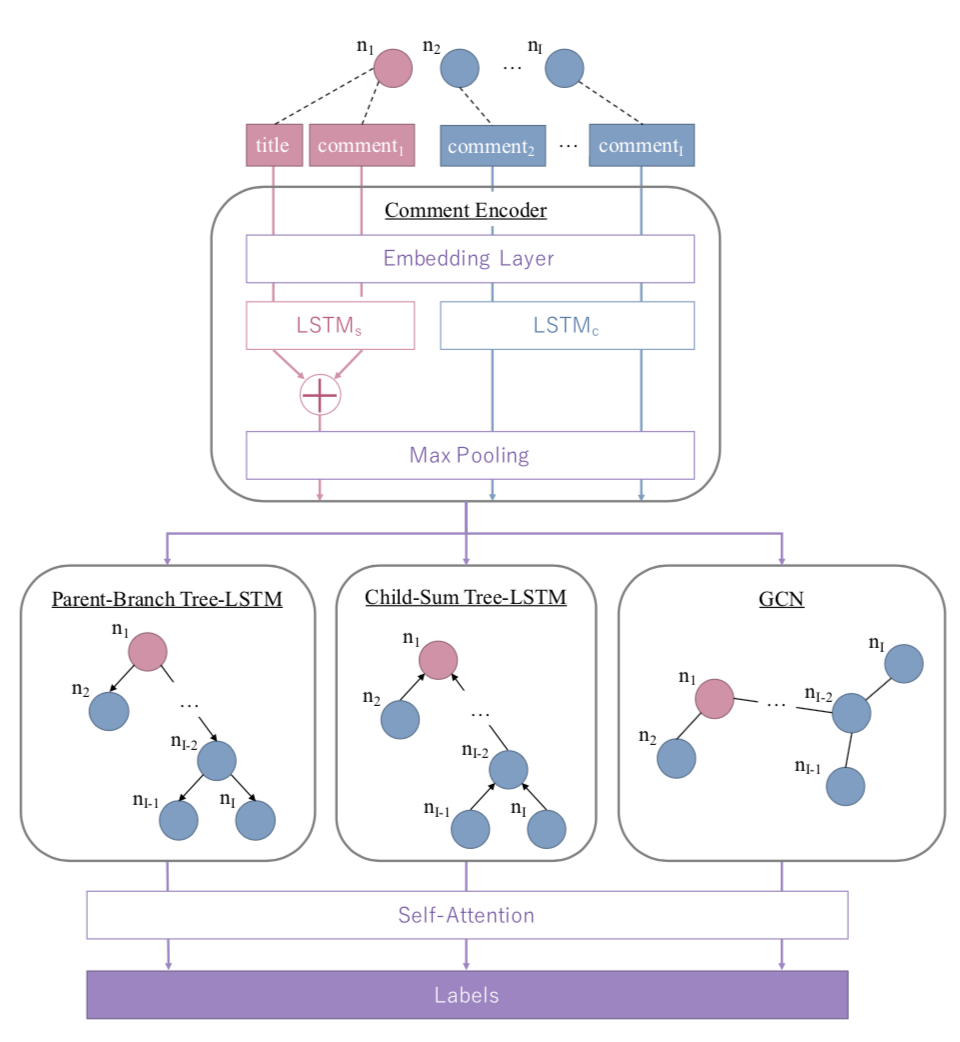
\includegraphics[width=0.7\textwidth]{images/related_work/integrating_tree.png}
  \end{center}
  \caption{The architecture of integrating tree-structures for text classification. The figures is taken from the original paper by Miura et al.~\cite{C18-1322}.}
  \label{fig:integrating_tree_structure}
\end{figure}

% Firstly und Secondly benutzen sehr viele Deutsche. First und Second ist auch voll okay.
\newpage

The aforementioned paper by Miura et al.~\cite{C18-1322} presented a new graph-based text classification architecture. Overall the architecture is quite complex as visualized in Figure~\ref{fig:integrating_tree_structure}. First, the comments are encoded into an internal representation. There is the different handling of the first comment (and its title) and all other comments. Second, the comments are given into three context-aware sub-networks before getting concatenating again. To evaluate the performance of their architecture, they conduct experiments on a research dataset of annotated Reddit comments by Zhang et al.~\cite{coarsediscourse}. For text representation, they train Word2vec on a millions of Reddit comments. They achieved higher results than previously reported. The Reddit comments are annotated for their role in a discourse. For instance whether a comment is question or answer. This setting is called \textit{discourse classification}.

Another related problem is \textit{stance detection}. In this field, it is about detecting whether a response to a statement is affirmative or opposing. For this, Kochkina et al.~\cite{kochkina2017turing} introduced Branch-LSTM. They worked with tweets and split the structure into branches. Branch gets created by iterating over all branch nodes of the discussion tree. For each leaf, one goes all the way to the root. This sequence is called branch. The branches are then given as input to the network. For representing the text, they also use Word2vec but average the word embeddings for each comment. A simple averaging is too limiting to capture the nuances of a text~\cite{rueckle:2018}.
 Stops words or commons words such as forms of `be' or `have' appear often and distort the whole meaning that should be added with word embeddings.
In addition, they use various other hand-crafted features to enrich the tweet representation. There exist various similar ideas by Zubiga et al.~\cite{C16-1230, ZUBIAGA2018273} which has several works for the conversation.
There is also a different problem setting of identifying sarcasm in text.
Ghosh et al.~\cite{W17-5523} identified the role of conversation in this domain.
But they only encoded one previous post for each other post.
This is quite limiting since a conversation spans among multiple comments.
In addition, research on user product reviews is related field.
In it, there are as well approaches that take the context of a product review into consideration.
For instance, Zheng et al.~\cite{Zheng:2017:JDM:3018661.3018665} encoded the product description as well as reviews with an LSTM respectively before combining the two sub-networks into a classifier.

So there exists quite a lot of work on news comments as well as incorporating the conversation for the classification. But all of them a rather simplistic text representation of traditional word embeddings. In the next section, we will give background information on how text representation are derived from language models. They show superior results on various NLP tasks.
